\documentclass[paper=a4, fontsize = 12pt, DIV = calc, twoside=off, parskip=full, numbers=noenddot]{scrbook}
\usepackage[utf8]{inputenc}
\usepackage[ngerman]{babel}
\usepackage{blindtext}
\usepackage{microtype}
\usepackage{hyperref}
\usepackage{csquotes}
\usepackage{glossaries}
\usepackage{graphicx}
\usepackage{fancyref}
\usepackage{subcaption}
\usepackage{wrapfig}
\usepackage{float}
\usepackage{svg}
\makeglossaries
\newglossaryentry{airflow-code-editor}{
name = airflow-code-editor,
description = {Airflow-code-editor ist ein open-source Plugin (Apache-2.0 Lizenz) für Airflow, welches das programmierbasierte Editieren und Erstellen von DAGs in der Weboberfläche von Airflow ermöglicht. \nolinkurl{https://github.com/andreax79/airflow-code-editor}}
}

\newglossaryentry{AppBuilder}{ %Hier sollte noch mehr hin wahrscheinlich
name = \textit{AppBuilder},
description = Flask-AppBuilder ist ein Development-Framework welches auf Flask basiert. Es wird von
Airflow ab Version 2.0.0 für die Darstellung der Weboberfläche verwendet.
\nolinkurl{https://github.com/dpgaspar/Flask-AppBuilder}}

\newglossaryentry{Op}{ %Hier sollte noch mehr hin wahrscheinlich und was ist hier die Formale Definition hab mich dran versucht
name = Op,
description = Der Server Operator ist ein Nutzer welcher Schreibzugriff auf die grundlegende Konfiguration der Anwendung hat. Er ist somit in der Lage die Konfiguration der Serverstruktur der
Anwendung zu ändern.}

\newglossaryentry{Codemirror}{
name = Codemirror,
description = {Ist ein Editor zum Bearbeiten von Code in Webbrowsern welcher auf JavaScript basiert. 
Er ist open-source und wird steht unter der MIT-Lizenz. \nolinkurl{https://github.com/codemirror/CodeMirror}}
%\nolinkurl{https://github.com/codemirror/CodeMirror}
}

\newglossaryentry{Apache Airflow}{
name = Apache Airflow,
description ={Open-source Workflow Management Plattform für Workflows}
}

\title{{WAMS}\\
{\Large{Workflow Application for Material Sciences}}\\
{Entwurfsdokument}}
\author{Dominik Siebelt \and Max Umbach 
        \and Maxim Besser \and Isabel Kraft \and Fabian Zürker}
\date{Dezember 2021}

\begin{document}

\maketitle
\newpage
\tableofcontents
\newpage

\chapter{Einleitung}
WAMS baut auf der Basis von \Gls{Apache Airflow} auf und erweitert bzw. ändert die Standardkonfiguration von Airflow ab, sodass der geforderte Funktionsumfang erreicht wird.
Dafür bringt WAMS ein eigenes Plugin mit, das weitere Webansichten und Operatoren einfügt.
Diese Ergänzungen ermöglichen es WAMS mehr Funktionalität über die Weboberfläche anzubieten.

Dass WAMS Airflow als Basis nutzt und darauf aufbaut, ergibt folgende Vorteile:
\begin{itemize}
    \item Die Funktionalität von Airflow bleibt erhalten, sodass WAMS ebenso mit dem Ökosystem von Airflow interagieren kann.
    \item Updates von Airflow können ohne Anpassung des WAMS-Plugins übernommen werden.
    \item Weite Teile der Deployment-Logistik Airflows werden übernommen.
\end{itemize}
Jedoch liefert Airflow noch nicht gesamten Funktionsumfang der von WAMS gefordert wird. Wie der geforderte Funktionsumfang erreicht wird, wird im Folgenden beschrieben.

%
%Dies ermöglicht das Apache Airflow unabhängig von WAMS aktualisiert werden kann.
%Dies verbessert die Erweiterbarkeit von WAMS durch die Installation von Airflow Plugins.
%Dies ermöglicht das WAMS erweiterbar ist durch die Installation von Airflow Plugins.
%Dies ermöglicht eine Verwendung von der aktuellen Airflow Version selbst bei updates.

\section{Paketstruktur}

%WAMS besteht aus zwei Hauptbestandteilen. In diesen sind Klassen mit ähnlichen Funktionen 
%zusammengefasst.
WAMS kann grob in zwei Bestandteile aufgeteilt werden:
\begin{itemize}
    \item Eine Airflow-Instanz mit spezieller Konfiguration
    \item Das eigene Plugin, welches die Weboberfläche von Airflow erweitert
\end{itemize}

Airflow bietet für Plugins eine eigene Schnittstelle an, die von WAMS genutzt wird, um eigene 
Webansichten hinzuzufügen. Da Airflow ab Version 2.0.0 für seine Weboberfläche und Nutzerverwaltung
das Flask AppBuilder Framework nutzt, werden die Ansichten von WAMS ebenso dieses Framework nutzen.

Für die Speicherung von Daten, die speziell von den Ansichten des WAMS-Plugin verwendet wird, bringt WAMS zusätzlich noch eine eigene Datenbank mit, die in einem eigenen Container läuft und über eine API von den Webansichten und Operatoren angesprochen wird.


Da WAMS eine Erweiterung von Airflow ist, werden unter anderem folgende Funktionen von Airflow übernommen:
\begin{itemize}
    \item Bestehende Weboberflächen
    \item Webserver
    \item Speicherung der Workflows
    \item Parametrierung der Workflows
    \item Datenbank für Metadaten
    \item Scheduling von Workflows
    \item Ausführung von Workflows
\end{itemize}
WAMS fügt zu Airflow Funktionen hinzu, die an verschiedene Komponenten Airflows anbinden und sie erweitern, wie in Grafik  \ref{fig:airflowÜbersicht} verdeutlicht wird. Aufgrund dieser Anknüpfung an verschiedenen Stellen, wird für das WAMS Plugin keine Model-View-Controller-Struktur verwendet.

\begin{figure}[H]
    \includegraphics[width=\textwidth]{Diagramme/Airflow übersicht.png}
    \caption{Anbindungsorte der Erweiterungen Airflows durch das WAMS Plugin. Farblich hervorgehoben sind die einzelnen Funktionspakete.\\ \tiny{Grundlegende Struktur Airflows übernommen von \nolinkurl{https://aws.amazon.com/de/blogs/machine-learning/build-end-to-end-machine-learning-workflows-with-amazon-sagemaker-and-apache-airflow/}}}
    \label{fig:airflowÜbersicht}
\end{figure}

%Da WAMS Airflow als Plugin erweitert und dieses an verschiedenen Stellen von Airflow anknüpft, wird für WAMS keine Model-View-Controller Struktur verwendet.
Zudem werden große Teile der Benutzeroberfläche von Airflow übernommen. 
Deswegen wird WAMS in Pakete aufgeteilt, welche jeweils einer Funktionalität von WAMS entsprechen. Diese Einteilung ermöglicht auch hohe Wiederverwendbarkeit der einzelnen Funktionen und verbessert so auch die Wartbarkeit.
%Da die Erweiterungen von WAMS an vielen Stellen des Modells von Airflow anbinden, wird für WAMS keine Model-View-Controller Struktur verwendet.

%Dabei liegt der Fokus auf einer Aufteilung in unterschiedliche Funktionen. 
%Das führt dazu, dass WAMS modular aufgebaut ist. 
%So können einzelne Funktionen von WAMS auch für andere ähnliche Plugins verwendet werden.
%Im Vergleich zur Aufteilung der Funktionen in mehrere Pakete ist dies durch die gewählte Paketstruktur einfach möglich.
%Es müssen lediglich die Pakete in ein anderes Plugin übernommen werden. 
Die Hauptaufgaben von WAMS liegen im Bereitstellen mehrere Funktionen in der Weboberfläche.
Folgende Pakete mit Funktionen stellt WAMS bereit:
\begin{itemize}
    \item Code Editor
    \item Result View
    \item Metadata Explorer
    \item Operators
    \item WAMSDatabase
\end{itemize}

\begin{figure}[h]
    \centering
    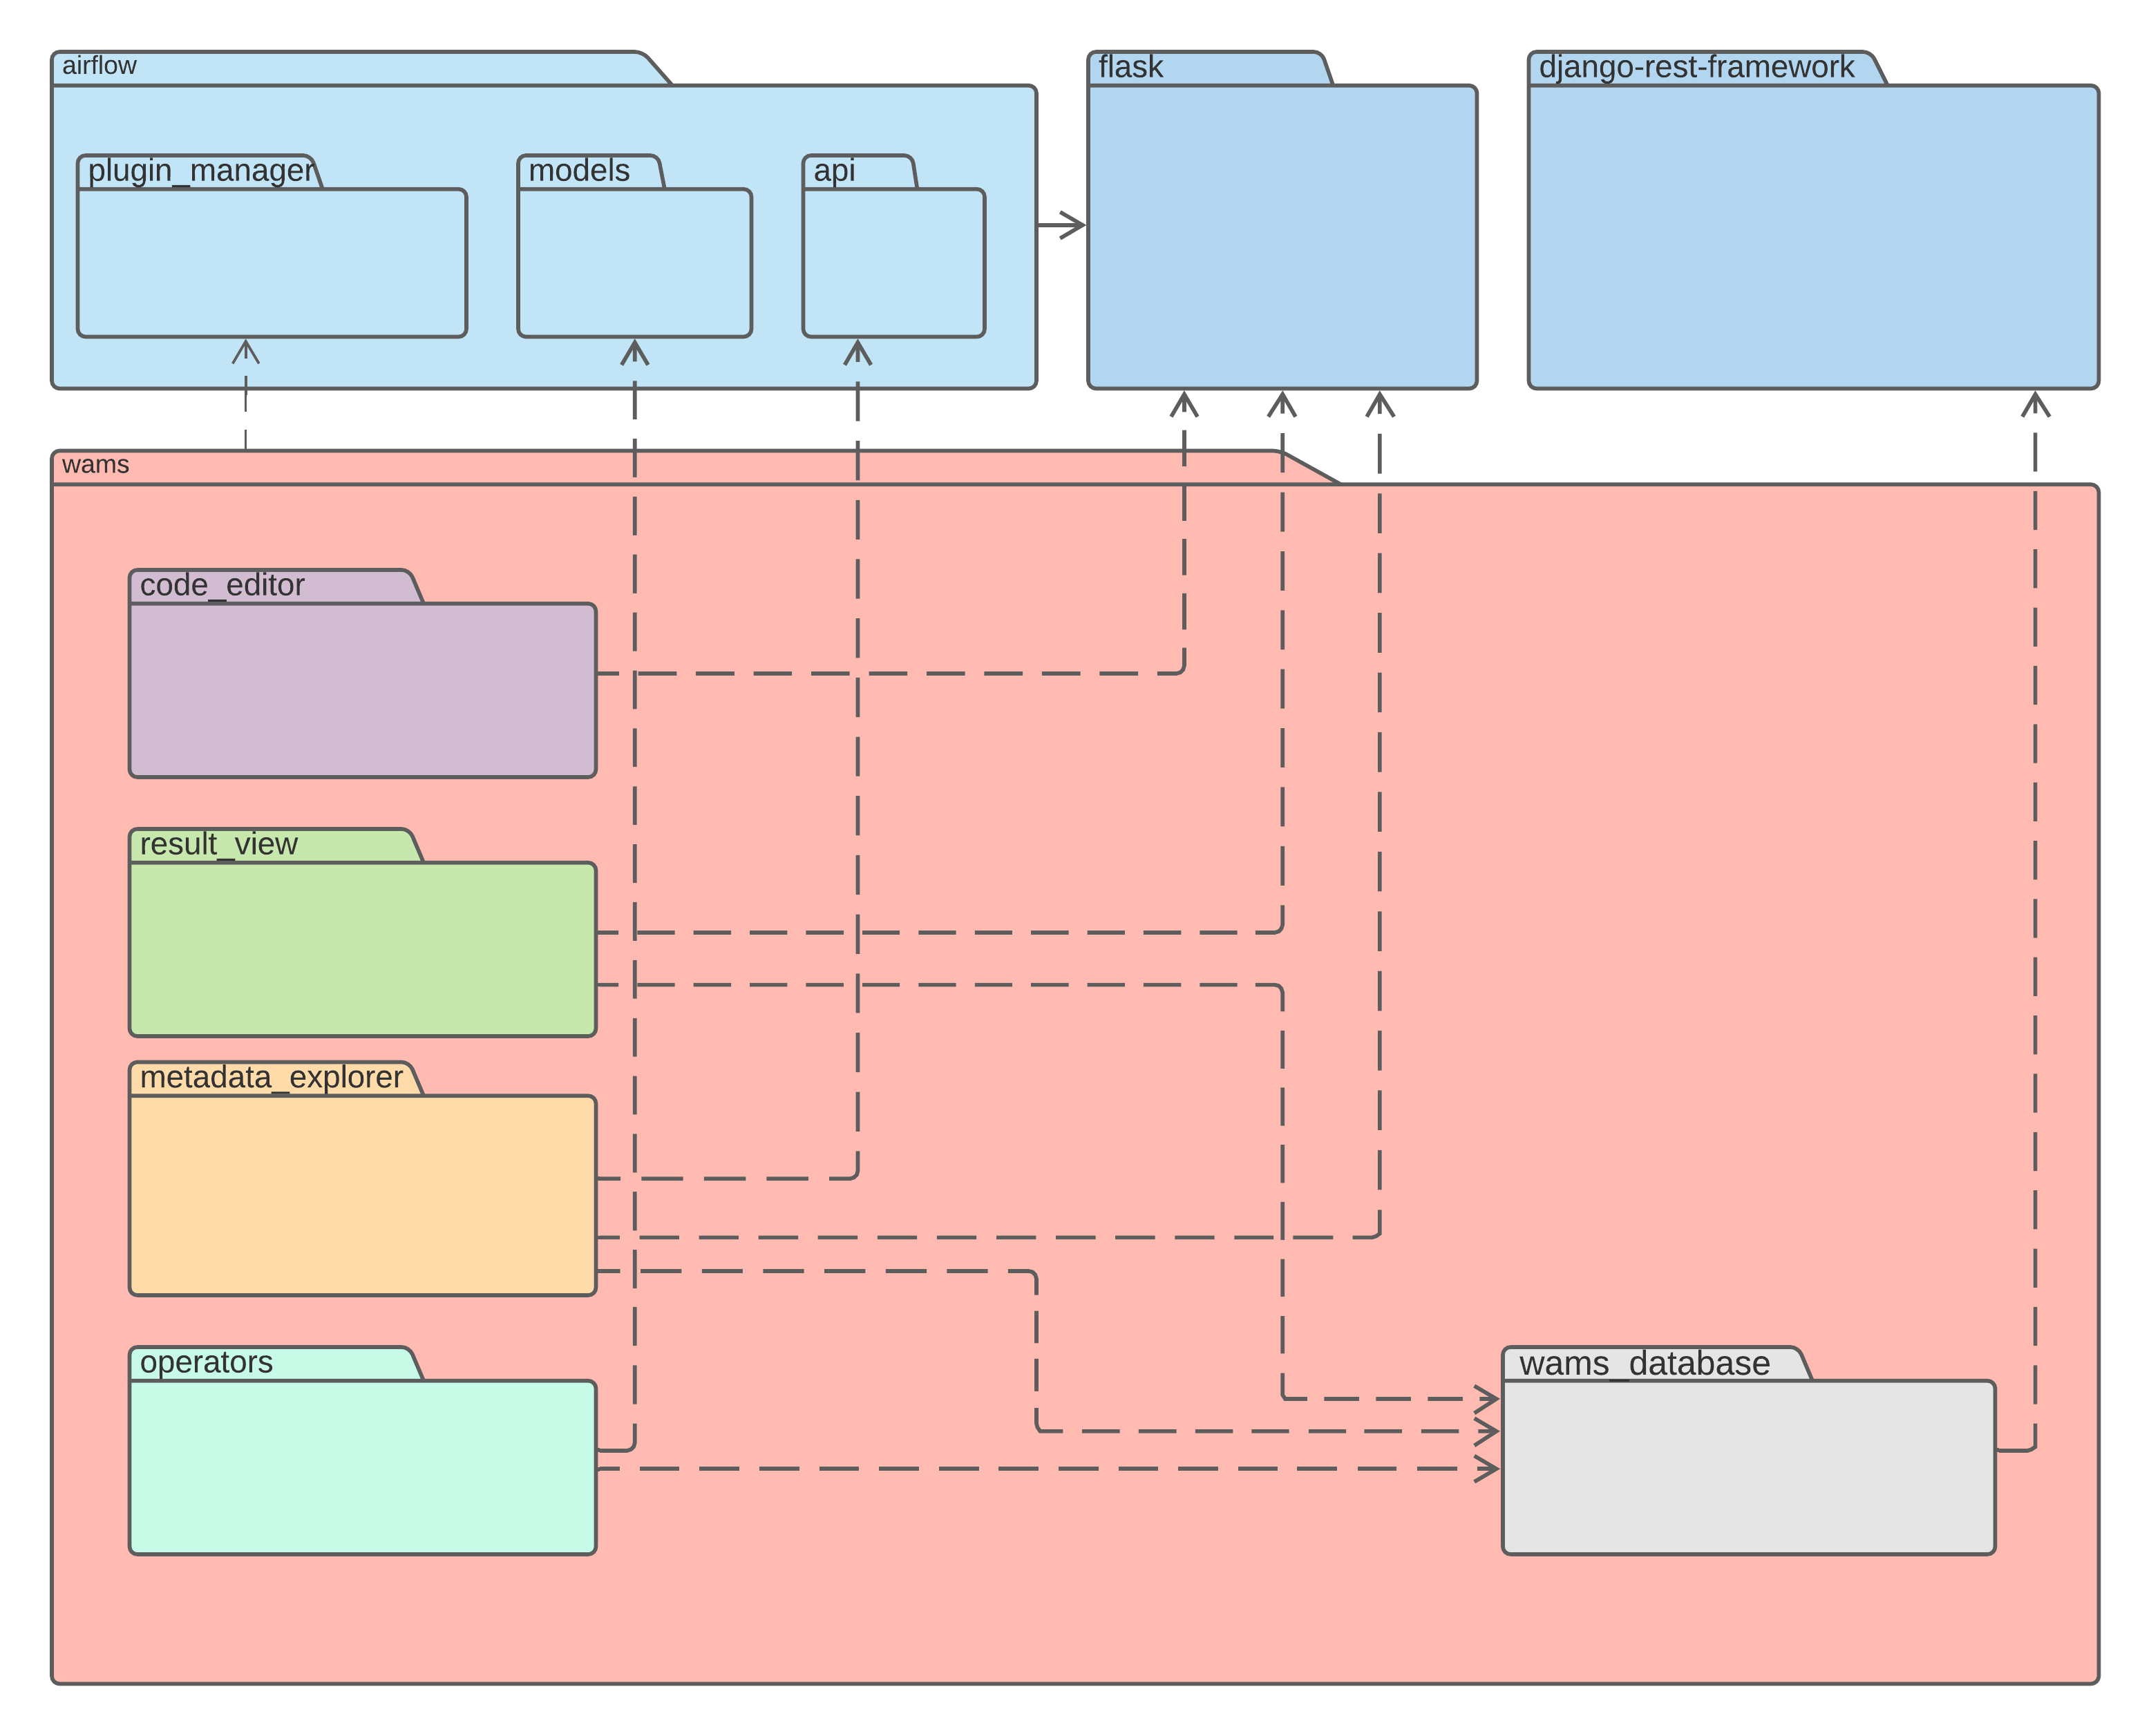
\includegraphics[width=\textwidth]{Diagramme/Paket.png}
    \caption{Paketdiagramm von WAMS}
    \label{fig:Paket}
\end{figure}

Diese Pakete werden in den nächsten Abschnitten einzeln behandelt.
Weiter greift WAMS auf mehrere Pakete innerhalb von Apache Airflow (\textit{airflow}) zu, insbesondere auf das Paket \textit{airflow.plugin\_manager} und auf das Paket \textit{airflow.api}. Das Paket \textit{airflow.plugin\_manager} liefert die Schnittstelle zur Einbindung des WAMS Plugins.
Das Paket \textit{airflow.api} enthält die Anwendungsprogrammierschnittstelle von Apache Airflow.

\subsection*{Code-Editor}
Der Code-Editor dient dazu den Python-Quellcode von Workflows in der Weboberfläche ändern zu können.
Hierbei wird das Airflow Plugin \gls{airflow-code-editor} von WAMS verwendet.

\subsection*{Result View}
Das Result View Paket erweitert die Weboberfläche von Airflow mit einem Tab zum Einsehen ausgewählter Ergebnisse und Zwischenergebnisse von Ausführungen von Workflows. 


\subsection*{Metadata Explorer}
Das Metadata Explorer Paket erweitert die Weboberfläche von Airflow durch einem Tab zum Einsehen der Metadaten einer Ausführung von Workflows. Die Metadaten werden über die Airflow API ermittelt.

\subsection*{Operators}
Das Operators Paket bündelt die in WAMS enthaltene Erweiterung der bereits in Apache Airflow existierenden Operatoren. 
In ihm sind Operatoren enthalten, die zu einer einfachen Anwendung von TGDS Workflows gedacht sind.
Außerdem ist ein Operator enthalten, der das Abspeichern von Ergebnissen und Zwischenergebnissen stark vereinfacht.

\subsection*{WAMSDatabase}
Das WAMSDatabase Paket ist zuständig für das Speichern von Daten im Zusammenhang mit Workflow-Instanzen.
\chapter{Design}
WAMS passt Airflow an die Bedürfnisse des Kunden an. WAMS liefert eine auf Experimente der Material- und Datenwissenschaften abgestimmte Konfiguration von Airflow, sowie zusätzlich benötigte Funktionalität in Form eines Airflow Plugins. Da die Webansicht von Airflow auf dem Flask Framework \gls{AppBuilder} basiert, bringt unser Plugin weitere Ansichten mit, die unter der Menüleiste eingefügt werden.

\section{Airflow Konfiguration}
\subsection{Nutzerverwaltung}
Airflow bietet standardmäßig fünf Nutzerklassen an auf die es alle Berechtigungen verteilt. Da WAMS nur drei Nutzerklassen hat, werden die Rechte wie folgt reduziert:
\begin{itemize}
    \item Admin: übernehmen die Rolle des \gls{Op} und erhalten für alle Bereiche
    Lese- und Schreibrechte. 
    \item Developer: erhalten Lese- und Schreibrechte für alle Bereiche, außer der Konfiguration von Airflow.
    \item Reviewer: erhält nur Leserechte.
\end{itemize}

Airflow übernimmt die Login-Seite von \gls{AppBuilder} und kann somit nach der Dokumentation von Flask \gls{AppBuilder} angepasst werden, um die Registrierung neuer
Nutzer anzubieten. Auch die neuen Ansichten, die von WAMS geliefert werden nutzen die 
Nutzerverwaltung von Flask \gls{AppBuilder}.

\section{Plugin}
Airflow bietet nativ noch nicht alle gewünschten Funktionalitäten. Daher bietet WAMS
noch drei weitere Ansichten um den gewünschten Funktionsumfang zu erreichen. Diese sind:
\begin{itemize}
    \item Editor-Ansicht: zum Editieren der DAG-Definitions-Dateien
    \item Result-Ansicht: zur Auflistung und Anzeigen der durch Workflows erstellte Dateien
    \item Metrics-Ansicht: zur Auflistung der ausgeführten Workflows-Instanzen 
    und den dazugehörigen Metadaten
\end{itemize}
Als zusätzliche Komponente bringt WAMS eine eigene Datenbank für die 
Speicherung der benutzerdefinierten Resultate und Zwischenergebnisse von Workflows-Instanzen und die dauerhafte Speicherung von Metadaten mit. Die Datenbank befindet sich in einem eigenen Container und kann von den anderen Ansichten über eine API angesprochen werden. %lebt? Sagt man das so?

\subsection{Editor-Ansicht}
Um das Editieren von Workflows in der Weboberfläche von Airflow zu ermöglichen, bedienen wir uns an dem bereits existierendem Plugin \gls{airflow-code-editor}. %Muss noch überarbeitet werden weiß nicht genau was wir da abgeändert haben
Dieses Plugin implementiert bereits eine Anzeige für die Ordnerstruktur und die Editierung von Textdateien in der Weboberfläche von Airflow.
Dabei nutzt es den Javascript Editor \gls{Codemirror}. Über die gewünschte Funktionalität hinaus bietet \gls{airflow-code-editor} zudem noch eine Git-Integration über die gleiche Weboberfläche an. %Diese Weboberfläche binden wir in unser Plugin ein, um dessen Funktionalität anzubieten. %wessen?


Um die Weboberfläche von \gls{airflow-code-editor} für unsere Anwendung zu nutzen, braucht es noch folgende Anpassungen:

\begin{itemize}
    \item Das Hauptverzeichnis wird von \verb!$AIRFLOW_HOME/! zu \verb!$AIRFLOW_HOME/dags/! geändert.
    \item In der Titelleiste von Airflow wird ein Reiter hinzugefügt, über den man auf die Weboberfläche des Plugins zugreifen kann.
    \item Die Zugriffsberechtigung auf die Weboberfläche muss von Admin auf Developer erweitert werden.
\end{itemize}

\subsection{Results-Ansicht}
Damit Nutzer von WAMS für einzelne Durchläufe eines Workflows jeweils Resultate abspeichern und über die Weboberfläche auf diese zugreifen können, bietet WAMS einen eigenen Operator (SaveResultsOperator) für die Speicherung von ausgewählten Dateien und eine weitere Webansicht für eine Ansicht der Ergebnisse.

\subsubsection{SaveResultsOperator}
Der Operator ist eine Unterklasse des BaseOperator von Airflow. Er nimmt als Argumente ein Verzeichnis, das er sichern soll oder eine Liste an Dateien, die gesichert werden sollen. Er kann am Schluss des Workflows ausgeführt werden, um ein Gesamtresultat zu speichern oder nach einzelnen Operatoren ausgeführt werden, um auch Zwischenresultate zu speichern.

Während seiner Ausführung baut er eine Verbindung mit der Datenbank von WAMS auf und legt die gewünschten Dateien in dieser ab. Der Operator übergibt der Datenbank neben den zu sichernden Dateien noch Informationen über den Workflow und der Workflow-Instanz, die den Operator ausführt, sodass die Datenbank die Dateien richtig zuordnen und eindeutig ablegen kann.


\subsubsection{Results-Webansicht}
Die Webansicht der erzeugten Ergebnisse wird mit Hilfe von Flask \gls{AppBuilder} erzeugt und enthält Komponenten, die die Workflows, Workflow-Instanzen und Workflowinstanzergebnisse aus der Datenbank abfragen und graphisch in der Weboberfläche darstellen können.


\subsection{Metadaten-Ansicht}
Da Airflow bereits eine API für den Zugriff auf Metadaten besitzt, wird die Metadaten-Ansicht von WAMS diese verwenden. 
Die Metadaten einer Workflowinstanz werden beim Löschen des zugehörigen Workflows oder beim Löschen der Workflowinstanz ebenfalls gelöscht. Um die Persistenz der Metadaten zu gewährleisten, werden die Metadaten einer Workflow-Instanz in der Datenbank von WAMS hinterlegt. Die Daten in der WAMS Datenbank sind dabei immutable und werden beim Löschen des Workflows nicht entfernt.

Die Aufgaben der Metadaten-Ansicht werden dabei wie folgt auf Klassen aufgeteilt:
Eine Klasse, die dafür zuständig ist, die Metadaten einer Worfklowinstanz, eine Liste von Instanzen eines Workflows und eine Liste von Workflows aus der WAMS-Datenbank zu holen. Diese Klasse hat dabei keinen Einfluss auf die GUI.
Zwei Klassen, die gemeinsam mit dem Flask-Blueprint dieser Ansicht für die graphische Darstellung der Workflows, Workflow-Instanzen und Metadaten verantwortlich sind. Eine Klasse ist dabei dafür zuständig, die Metadaten, welche als .json Datei vorliegen, graphisch darzustellen.

\subsection{WAMS-Datenbank}
Airflow nutzt bereits eine Datenbank für die Speicherung der Metadaten der Ausführungen von Workflows. Folgende Beschränkungen führen dazu, dass die Datenbank nicht ohne Anpassung von WAMS übernommen werden kann:
\begin{itemize}
    \item Die Metadaten gelöschter Workflows werden nicht erhalten.
    \item Es gibt keine Möglichkeit Dateien als Resultat von Workflows zu sichern.
\end{itemize}

Somit dient die WAMS-Datenbank sowohl als ein Speicher für die Ergebnisse und Zwischenergebnissen von Workflow-Ausführungen als auch eine Erweiterung der Airflow-Datenbank. Die WAMS-Datenbank wird Über eine API-Klasse, die POST- und GET-Methoden anbietet, angesprochen. Diese Klasse trifft abhängig von der Anfrage die Entscheidung, ob Metadaten oder Resultate einer Workflow-Instanz angefragt werden und delegiert die Beschaffung an andere Klassen.

Wird eine Datei angefordert, die Ergebnis einer Workflow-Instanz war, wird diese Anfrage an
die ResultHandler-Klasse weitergeleitet. Die ResultHandler-Klasse speichert die Ergebnisse
nach der dazugehörigen Workflow-Instanz in einem Verzeichnis und beschafft diese auf
Anfrage. Dabei werden gleichzeitig die Metadaten für die ausführende Workflow-Instanz
in einer MySQL-Datenbank gespeichert.

Wird eine Anfrage nach Metadaten zu einer Workflow-Instanz gestellt, wird diese 
MetricsGetter weitergeleitet. MetricsGetter versucht zunächst eine Anfrage über die
Airflow-Datenbank aufzulösen. Falls diese Anfrage jedoch erfolglos war, wird eine weitere
Anfrage an die eigene MySQL-Datenbank gestellt. Somit besteht auch nach Löschung eines 
Workflows die Möglichkeit auf Metadaten gelöschter Workflows zuzugreifen. Somit ist das Prinzip der Transparenz eingehalten, da für den Anwender nicht ersichtlich ist, aus welcher Datenbank die Informationen und Ergebnisse stammen, aber auch sichergestellt wird, dass immer die aktuellsten und korrekte Ergebnisse geliefert werden.
\chapter{Klassenbeschreibung}
\subsection{WAMSPlugin}
Main Class of the WAMS Plugin for Airflow. Ties together the other Classes in the plugin and implements the AirflowPlugin interface.
%Wrapper Klasse die die Hauptlogik des Plugins enthält und das AirflowPlugin interface implementiert.

\subsection{flask\_appbuiler.BaseView}
Klasse die für das Anzeigen der einzelnen Komponenten des Plugins veranwortlich ist.

\section{CodeEditor}
\subsection{CodeEditorController}
Class that connects the Code editor plugin with the WAMS plugin and connection to Git and Tree.

\subsection{CodeEditorView}

\subsection{ResultView}
Class that is responsible for the apperance of the Results part of the workflows. 

\subsection{MetricsView}
Klasse die Darstellung von der Metadaten Ansicht in der Anwendung zuständig ist. 
Die Klasse erweitert flask\_appbuiler.BaseView.

\subsubsection{MetricsFetcher}
Class that is responsible for the fetching of the Metadata of a specific workflow from the Airflow Database.

\subsection{Json View}
Klasse die für das Darstellen von Json Datein zuständig ist.

\section{Operators}
\subsection{PingPongOperator}
%Operator class used for dynamically created tasks like the theory guided maschine learning modell.
This operator receives two python callables. It executes both of them alternating as often as specified in the repetition parameter of its \textit{\_\_init\_\_()} method. The results of the callables can be used as input parameters for each repetition to allow increasing accuracy of the model. The first callable can be started with paramters also passed in the \textit{\_\_init\_\_()} method.


\subsection{TriggerTillSatOperator}
This operator receives two python callables. In opposition to the \textit{PingPongOperator} the number of repetition is not set via the \textit{\_\_init\_\_()} method but can change dynamically. The first callable triggers the second one every time the second one has finished its work until it is satisfied. The threshold value deciding if the second callable should be run again can also be passed in the \textit{\_\_init\_\_()} method. The first callable receives the return values of the second one after every run of the second one.


\section{Ergebnispaket}
\subsection{ResultsExplorerView}
Klasse die für das Anzeigen der Ergebnisse in dem Dateiexplorerer zuständig ist.
Die Klasse erweitert flask\_appbuiler.BaseView.


\section{Klassen von außerhalb} %Airflow, code editor etc
Klassen die nicht von uns Geschrieben wurden/werden aber trotzdem für den Aufbau relevant sind da diese erweitert werden oder referenziert werden.

\subsection{AirflowPlugin interface}
Das Interface von Airflow das implementiert werden muss damit ein Plugin für Airflow nutzbar ist. Wird von WAMSPlugin implementiert

\subsection{BaseOperator}
Klasse von Airflow die einen BaseOperator von Airflow definiert. 

\subsection{Airflow API}
API von Airflow

\subsection{List Dags (resource)}
Resource die eine liste von allen DAGs ist.

\subsection{List Dag runs (resource)}
Resource die eine liste von allen DAG runs ist. 

\subsection{flask.Blueprint}
Klasse von flask mit der Templates gehandhabt werden können.

\subsection{code\_editor\_plugin\_blueprint: Blueprint}
Implementiert die flask.Blueprint Klasse/das Interface. 



\subsubsection{templates}

\subsubsection{static}

\subsubsection{utils.py}
%Python Library Klasse 
\subsubsection{commony.py}

\subsubsection{tree.py}


\include{Kapitel/Abläufe}
\chapter{Anhang}
\blindtext

%Exportieren von Dag definition files über Applikation exportieren
%Braucht man um Workflow Instanzen sowie Workflows zu erportieren
\end{document}

%PRIO1
%Hochladen von Dateien (Config)
%Dateiexplorer und Festlegen von Orten für Ergebnisse

%PRIO2 TODO
%Liveanzeige von Logdateien